%
% lncover.tex -- Cover für Vorlesungsnotizen
%
% (c) 2018 Prof Dr Andreas Müller, Hochschule Rapperswil
%
\documentclass[11pt]{standalone}
\usepackage{tikz}
\usepackage{times}
\usepackage{geometry}
\usepackage[utf8]{inputenc}
\usepackage[T1]{fontenc}
\usepackage{times}
\usepackage{amsmath,amscd}
\usepackage{amssymb}
\usepackage{amsfonts}
\usepackage{german}
\usepackage{txfonts}
\usepackage{ifthen}
\usepackage{qrcode}
\usetikzlibrary{math}

\begin{document}
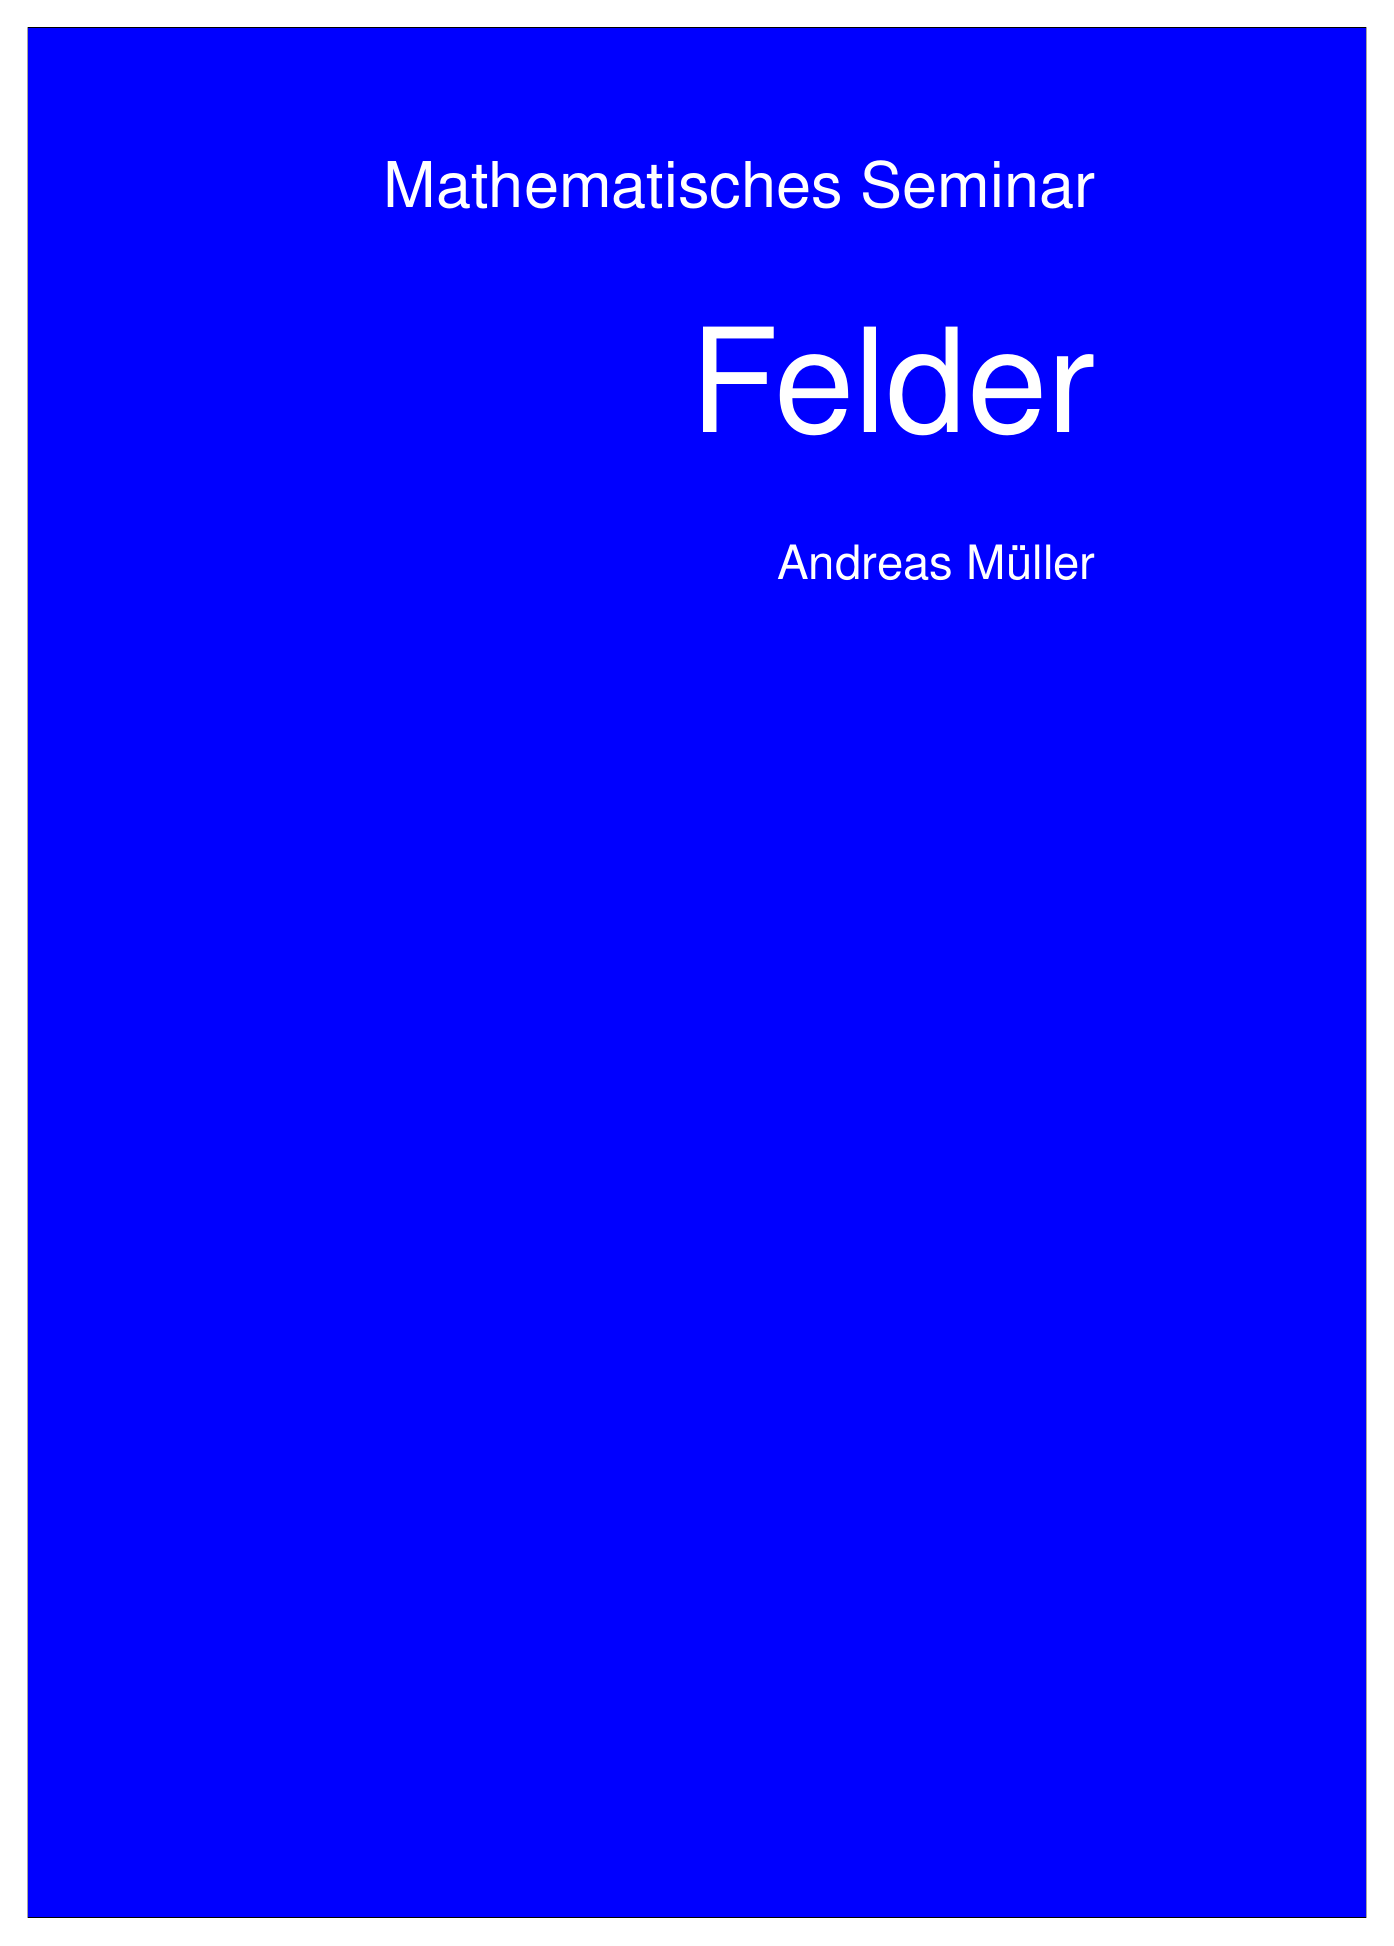
\begin{tikzpicture}[>=latex,scale=1]

\def\bogenbreite{17.0}
\def\bogenhoehe{24.0}

\clip (0,0) rectangle ({\bogenbreite},{\bogenhoehe});

\draw[fill=blue] (0,0) rectangle ({\bogenbreite},{\bogenhoehe});

\node at (7.5,22)
	[color=white,scale=1]
	{\hbox to\hsize{\hfill%
	\sf \fontsize{24}{24}\selectfont Mathematisches Seminar}};

\node at (7.5,19.5)
	[color=white,scale=1]
	{\hbox to\hsize{\hfill%
	\sf \fontsize{55}{55}\selectfont Felder}};

\node at (7.5,17.2)
	[color=white,scale=1]
	{\hbox to\hsize{\hfill%
	\sf \fontsize{18}{18}\selectfont Andreas Müller}};

\end{tikzpicture}
\end{document}
